
\chapter{同步性改善全局最优的递归自修复算法}

\section{自修复算法目标}
根据上文所述,当多机器人编队中度较高的机器人出现缺失时,会导致编队同步性下降。假设在图\ref{fig:修复路径对比}中,空缺位置表示出现机器人缺失,记缺失机器人为$R_f$,则缺失机器人的度$d_{R_f} = 6$。由引理\ref{lem:degree_syn}可知。若用度小于$d_{R_f}$的机器人修复此缺失机器人,则会提高编队的同步性。若最终修复机器人为$R_r$,度为$d_{R_r}$。则$d_{R_f}-d_{R_r}$的值越大,同步性改善效果越好。因此,如果用编队中度最小的机器人去修复缺失机器人则会使同步性改善效果最优。
\begin{figure}[!htbp]
	\centering
	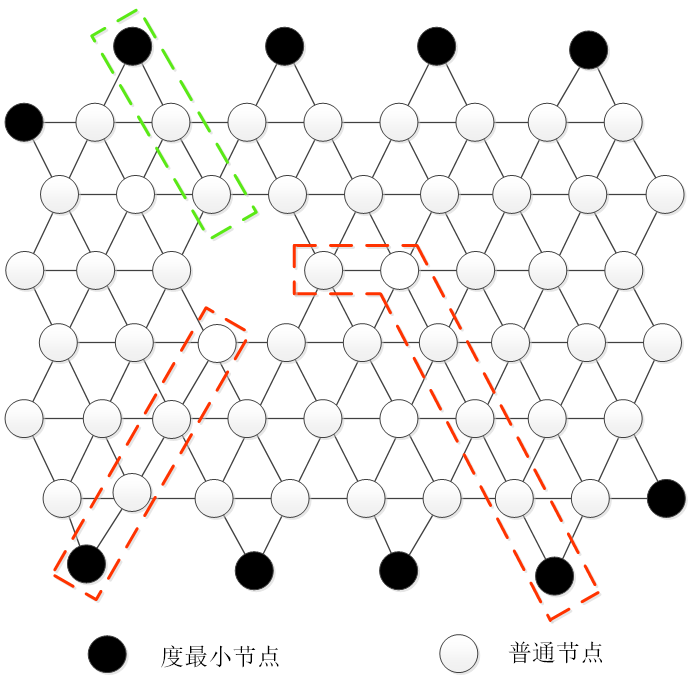
\includegraphics[width=8cm,height=8cm]{chapter3/figure3-1.png}
	\bicaption[fig:修复路径对比]{不同修复路径对比}{不同修复路径对比}{Fig}{The comparation of different repairing paths.}
\end{figure}

如何找到一条从缺失机器人到度最小机器人的修复路径是本文算法的主要内容。在这里修复路径定义为从缺失机器人邻居中的某个机器人到编队中度最小机器人所经过的机器人序列$\{R_1,R_2,\dots,R_{k-1},R_k\}$。修复路径上的机器人成为修复机器人,其中$R_1$为缺失机器人邻居中的某个机器人,$R_k$为编队中某个度最小的机器人。在图\ref{fig:修复路径对比}中,每一个虚线框中的机器人序列都属于一条修复路径。从图中可以看到不同的修复路径包含的修复机器人个数不同。定义包含修复机器人个数最少的修复路径为最优修复路径,图中绿色虚线框内的修复路径即为一条最优修复路径。如果一条修复路径中的修复机器人序列为$\{R_1,R_2,\dots,R_{k-1},R_k\}$,则对应的递归自修复步骤如下:\\
\indent (1)从缺失机器人的邻居中选择一个修复机器人$R_1$,$R_1$去填补缺失机器人留下的空缺位置,并与缺失机器人邻居重新建立。\\
\indent (2)$R_1$从其邻居中选择一个修复机器人$R_2$用来填补$R_1$移动后留下的空缺位置,并与$R_1$的邻居重新建立连接。\\
\indent (3)重复上述过程,直到编队中的度最小机器人$R_k$填补了$R_{k-1}$留下的空缺位置。\\
第(3)步结束后,整个修复机器人序列的递归自修复过程结束。在这一过程中,修复机器人的空间位置和网络邻居变化如下:\\
空间位置变化:\\
\begin{equation}
	P_{R_i} = 
	\begin{cases}
		P_{R_f}, & i=1 \\
		P_{R_{i-1}}, & 1 < i \leq k
	\end{cases}
\end{equation}
网络邻居变化:\\
\begin{equation}
	N_e(R_i) = 
	\begin{cases}
		N_e(R_f) - R_i + R_{i+1}, & i = 1 \\
		N_e(R_{i-1}) - R-i + R_{i+1}, & 1<k \leq k
	\end{cases}
\end{equation}

由于本文采用递归自修复方式实现分布式控制,因此编队中机器人无法知道距离缺失机器人最近的度最小机器人在哪里。即如何找到一条最优的修复路径?

\section{梯度的引入与分析}
根据前人的研究,梯度常被用于通过邻居之间的交互估计分布式距离的一种手段\supercite{SciencePaper,nagpal2003organizing,stoy2006using,rubenstein2012kilobot,meng2011autonomous,terada2008automatic},多应用于有限通信范围下的多传感器网络\supercite{nagpal2003organizing}以及多机器人自组织行为\supercite{SciencePaper,stoy2006using}等问题。主要是通过个体间的局部交互来控制整体。文献\parencite{SciencePaper,stoy2006using,rubenstein2012kilobot,terada2008automatic}中,首先定义一个梯度种子节点,由种子节点产生一个初始梯度值,接下来梯度值从种子节点开始扩散,邻居节点接收到扩散的梯度信息后更新自己的梯度信息,一般情况是如果接受到的梯度小于自身已有的梯度值(自身梯度值初始化为一个很大的数),则更新自身梯度值,否则维持自身梯度值不变。接下来再将自身保持的梯度值向邻居扩散,重复此过程,最终整个网络会形成稳定的梯度分布。每个机器人利用自身的梯度信息便可以知道自己与梯度种子节点的距离。图\ref{fig:Gradient_Sample}展示的是文献\parencite{SciencePaper}中的梯度应用示例。在多机器人自组织行为中,预先指定一个梯度种子节点的梯度值以及它的全局坐标,利用梯度扩散与更新过程在网络中形成稳定的梯度分布,在扩散与更新过程中,每个机器人只与它相邻的机器人通信。最终每个机器人根据自身的梯度值以及梯度种子节点的全局坐标估计出自己的全局坐标,从而完成自组织任务。
\begin{figure}[!htbp]
	\centering
	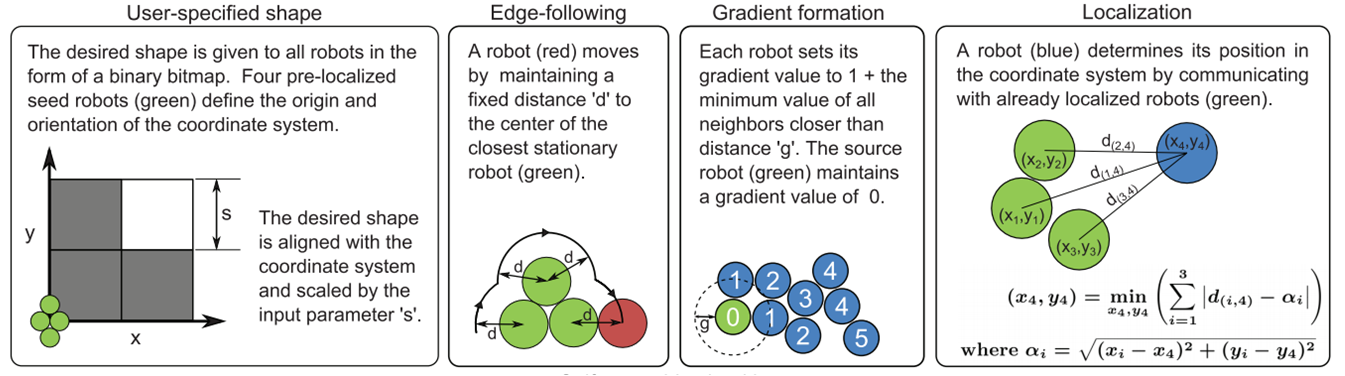
\includegraphics[width=12cm,height=3cm]{chapter3/figure3-2.png}
	\bicaption[fig:Gradient_Sample]{应用梯度实现多机器人自组织行为}{应用梯度实现多机器人自组织行为}{Fig}{Using Gradient to implement multi-robot self-assembly behaviors.}
\end{figure}

为对比有无梯度信息在多机器人编队自修复中的差别,文献\parencite{张飞2008移动机器人覆盖问题的研究}和文献\parencite{liu2015gradient}分别实现了无梯度和有梯度的多机器人编队自修复算法。在文献\parencite{张飞2008移动机器人覆盖问题的研究}中,编队中机器人缺失后仅根据邻居机器人的度的信息选择修复机器人,选取规则为:\\
\indent 1) 如果缺失机器人$R_f$的邻居$R_j \in N_e(i_f)$的度小于$R_f$的度,即$d_{R_j} \leq d_{R_f}$,则机器人$R_j$成为缺失机器人$R_f$的候选修复机器人。所有满足条件的候选修复机器人组成集合:\\
\begin{equation}
	C(R_f) = \{ R_j | d_{R_j} \leq d_{R_f}, R_j \in N_e{R_f} \} 
\end{equation} 
\indent 2) 在集合$C(R_f)$中选择度最小的机器人作为缺失机器人$R_f$的修复机器人,如果存在多个度最小机器人,则随机选择一个作为修复机器人。\\

本文中称此算法为随机递归自修复算法。图\ref{fig:Random_self-healing}中展示了在多机器人编队拓扑中出现一个机器人丢失,应用随机自修复算法进行修复的几种情况。
\begin{figure*}[!htbp]
	\centering
	\begin{tabular}{cc}
		\subfigure[]{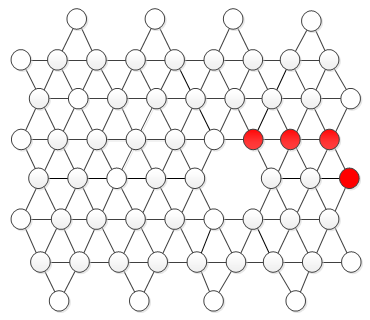
\includegraphics[width=4cm,height=3.5cm]{chapter3/figure3-3a.png}} & 
		\hspace{2cm}
		\subfigure[]{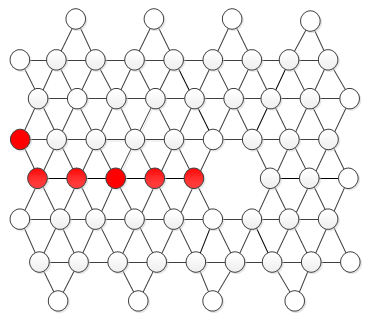
\includegraphics[width=4cm,height=3.5cm]{chapter3/figure3-3b.png}} \\

		\subfigure[]{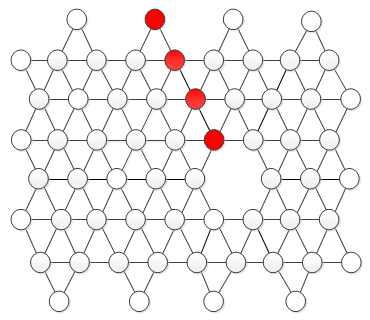
\includegraphics[width=4cm,height=3.5cm]{chapter3/figure3-3c.png}} & 
		\hspace{2cm}
		\subfigure[]{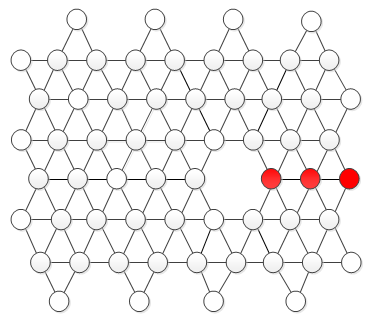
\includegraphics[width=4cm,height=3.5cm]{chapter3/figure3-3d.png}} 
	\end{tabular}
	\bicaption[fig:Random_self-healing]{随机递归自修复算法}{随机递归自修复算法,空缺位置表示此处机器人丢失,红色节点表示修复机器人}{Fig}{Random-based recursive self-healing algorithm.}
\end{figure*}

从图中可以看出随机递归自修复算法在实现自修复时选出的修复路径有很大的随机性,且不同的修复路径性能差异较大。造成这种现象的原因主要是在修复机器人选取规则2中,当存在多个满足条件的候选修复机器人时随机选择其中一个,由此对修复路径造成很大的随机性。

为避免在自修复中引入过大的随机性,本研究团队在之前工作中引入梯度,大大降低了随机性,提高了自修复算法的性能。如图\ref{fig:Gradient_self-healing}所示,是在编队网络中引入梯度,形成稳定的梯度分布,算法中与前人不同的是并不事先指定一个梯度种子节点,而是节点根据自己在拓扑网络中邻居数量判断自己是否为梯度种子节点(又称为梯度源节点)。修复机器人选取规则为:\\
\indent 1)在缺失机器人$R_f$的邻居中选择度不大于缺失机器人度的机器人作为候选修复机器人。\\
\indent 2)选择候选修复机器人集合中度最小的机器人作为修复机器人。\\
\indent 3)如果存在多个度最小的候选修复机器人,则选择梯度值最小的机器人作为修复机器人。\\
\indent 4)如果存在多个度最小且梯度值最小的候选修复机器人,则从中随机选择一个机器人作为修复机器人。\\
图\ref{fig:Gradient_self-healing}是引入梯度后的自修复情况,本文称此算法为基于梯度的递归自修复算法。
\begin{figure*}[!htbp]
	\centering
	\begin{tabular}{cc}
		\subfigure[]{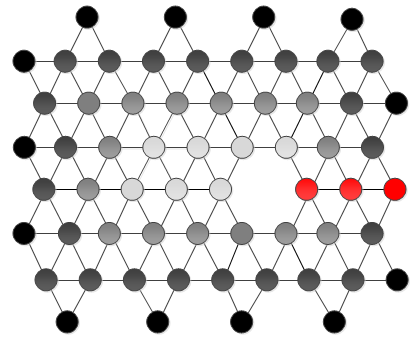
\includegraphics[width=4cm,height=3.5cm]{chapter3/figure3-4a.png}} & 
		\hspace{2cm}
		\subfigure[]{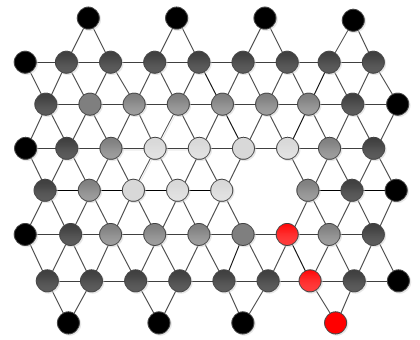
\includegraphics[width=4cm,height=3.5cm]{chapter3/figure3-4b.png}} \\
		
		\subfigure[]{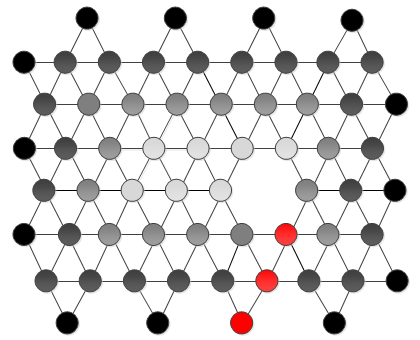
\includegraphics[width=4cm,height=3.5cm]{chapter3/figure3-4c.png}} & 
		\hspace{2cm}
		\subfigure[]{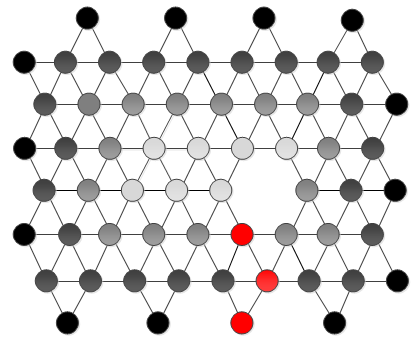
\includegraphics[width=4cm,height=3.5cm]{chapter3/figure3-4d.png}} 
	\end{tabular}
	\bicaption[fig:Gradient_self-healing]{基于梯度的递归自修复算法}{基于梯度的递归自修复算法,颜色的深浅表示梯度值的大小,颜色越深梯度值越小。黑色节点为梯度源节点。空缺位置表示此处机器人丢失,红色节点表示修复机器人}{Fig}{Gradient-based recursive self-healing algorithm, the shade means different gradient value, the deeper the color, the bigger the gradient value, the vacancy means failure robot and red nodes means repairing robots.}
\end{figure*}
从图中可以看到,引入梯度后修复路径的随机性降低很多,且修复路径是一条最短的修复路径。但是这里存在局部极小问题,在图\ref{fig:Gradient_self-healing}(a)中修复机器人序列中最后的梯度源节点机器人的度并不是全局最小。因此根据引理\ref{lem:degree_syn},同步性改善并不是全局最优。

本文借鉴前人的做法,在多机器人编队自修复算法中利用梯度分布式估计机器人与度最小机器人的距离,从而找到最优的修复路径。但为避免局部极小的问题,编队在梯度扩散与更新过程中所传播的信息不只是梯度信息还包括梯度源节点的度的信息,从而将局部度极小节点而非全局度最小节点更新。下文会具体分析这一过程。

\section{同步性改善全局最优自修复算法}

\subsection{算法框架}
总结前人研究的经验,本文设计了一种能够实现同步性改善全局最优的递归自修复算法。本文算法可以在编队中每个机器人个体上独立运行,从而实现完全分布式控制。本文算法主要根据在自修复过程中个体机器人本身在不同情况下所执行的任务的不同分为5种状态,分别为初始状态、梯度源节点状态、非梯度源节点状态、候选修复状态以及修复状态。在多机器人编队开始运行之后,编队中的机器人首先处于初始状态,通过执行梯度源节点生成算法判断自身是否为梯度源节点,若满足满足梯度源节点条件,则状态转移到梯度源节点状态,否则,状态转移到非梯度源节点状态。处于梯度源节点状态和非梯度源节点状态的机器人进行梯度的更新与扩散,最终在编队网络中形成稳定的梯度分布。编队在出现机器人缺失后执行修复的过程是建立在稳定的梯度分布基础之上的。形成稳定的梯度分布之后,当编队中出现机器人缺失时,缺失机器人的邻居检测到邻居中出现机器人缺失,则由当前状态转移到候选修复状态,所有处于候选修复状态下的机器人采用本文提出的竞选机制进行竞选以决出最终的修复机器人。竞选胜出的机器人状态转移到修复状态,处于修复状态的机器人将修复状态进行传递,知道度最小机器人状态转移到修复状态。图\ref{fig:FSM}的FSM图描述了机器人各个状态之间的转换关系。下文会结合编队拓扑给出各个状态更详细的分析。
\begin{figure}[!htbp]
	\centering
	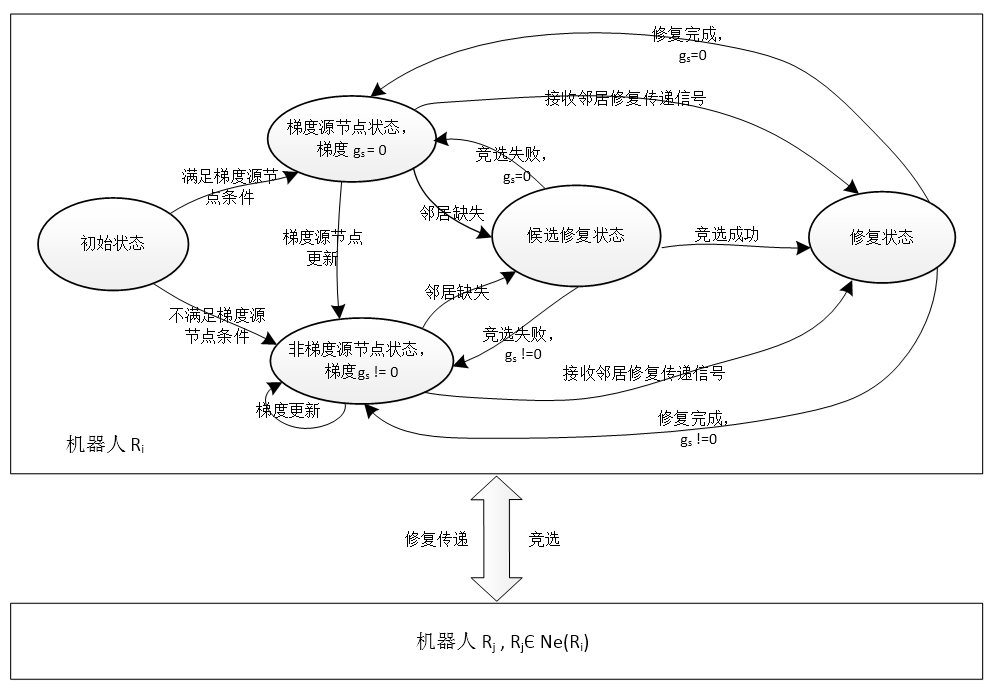
\includegraphics[width=14cm,height=10cm]{chapter3/figure3-5.png}
	\bicaption[fig:FSM]{同步性改善全局最优自修复算法状态转换图}{同步性改善全局最优自修复算法状态转换图}{Fig}{The FSM for the proposed algorithm.}
\end{figure}

\subsection{初始状态}

\subsection{梯度源节点状态}

\subsection{非梯度源节点状态}

\subsection{候选修复状态}

\subsection{修复状态}
